\documentclass[letterpaper]{article}
\usepackage[margin=1in]{geometry}
\usepackage{amsmath,amssymb}
\usepackage{tikz}

\newcommand{\aln}[1]{\begin{align*} #1 \end{align*}} % fast align

\begin{document}

\tikzstyle{every node}=[circle, draw, fill=black!50, inner sep=0pt, minimum width=4pt]

\title{Gr\"obner Bases of some Undirected Graphs Using an Alternate Cycle Encoding}
\author{Max Comstock}
\date{Summer 2014}
\maketitle

\section{Three Vertices with One Hamiltonian Cycle}

\begin{center}
  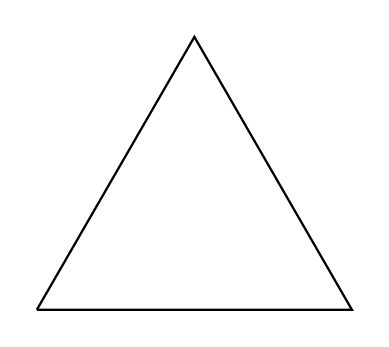
\begin{tikzpicture}[thick,scale=0.8]
    \draw (0,0) node {} -- (5,0) node {} -- (60:5) node {} -- (0,0);
  \end{tikzpicture}
\end{center}
\aln{
	y_1 + y_2 + y_3 - 3&= 0\\
	y_1(y_1 - 1) &= 0\\
	y_2(y_2 - 1) &= 0\\
	y_3(y_3 - 1) &= 0\\
	(x_1 - 1)(x_1 - 2)(x_1 - 3) &= 0\\
	(x_2 - 1)(x_2 - 2)(x_2 - 3) &= 0\\
	(x_3 - 1)(x_3 - 2)(x_3 - 3) &= 0\\
	y_1 (x_1 - y_2 x_2 + y_2)(x_1 - y_2 x_2 - y_2(3-1))(x_1 - y_3 x_3 + y_3)(x_1 - y_3 x_3 - y_3(3-1)) &= 0\\
	y_2 (x_2 - y_1 x_1 + y_1)(x_2 - y_1 x_1 - y_1(3-1))(x_2 - y_3 x_3 + y_3)(x_2 - y_3 x_3 - y_3(3-1)) &= 0\\
	y_3 (x_3 - y_1 x_1 + y_1)(x_3 - y_1 x_1 - y_1(3-1))(x_3 - y_2 x_2 + y_2)(x_3 - y_2 x_2 - y_2(3-1)) &= 0
}
\aln{
	\{x_3^3-6x_3^2+11x_3-6, x_2^2+x_2x_3-6x_2+x_3^2-6x_3+11, x_1+x_2+x_3-6, y_3-1, y_2-1, y_1-1\}
}


\newpage

\section{Four Vertices with One Hamiltonian Cycle}
\begin{center}
  \begin{tikzpicture}[thick,scale=0.8]
    \draw (0,0) node {} -- (5,0) node {} -- (5,5) node {} -- (0,5) node {} -- (0,0);
  \end{tikzpicture}
\end{center}
\aln{
	y_1 + y_2 + y_3 + y_4 - 4 &= 0\\
	y_1(y_1 - 1) &= 0\\
	y_2(y_2 - 1) &= 0\\
	y_3(y_3 - 1) &= 0\\
	y_4(y_4 - 1) &= 0\\
	(x_1 - 1)(x_1 - 2)(x_1 - 3)(x_1 - 4) &= 0\\
	(x_2 - 1)(x_2 - 2)(x_2 - 3)(x_3 - 4) &= 0\\
	(x_3 - 1)(x_3 - 2)(x_3 - 3)(x_3 - 4) &= 0\\
	(x_4 - 1)(x_4 - 2)(x_4 - 3)(x_4 - 4) &= 0\\
	y_1 (x_1 - y_2 x_2 + y_2)(x_1 - y_2 x_2 - 3y_2)(x_1 - y_4 x_4 + y_4)(x_1 - y_4 x_4 - 3y_4) &= 0\\
	y_2 (x_2 - y_1 x_1 + y_1)(x_2 - y_1 x_1 - 3y_1)(x_2 - y_3 x_3 + y_3)(x_2 - y_3 x_3 - 3y_3) &= 0\\
	y_3 (x_3 - y_2 x_2 + y_2)(x_3 - y_2 x_2 - 3y_2)(x_3 - y_4 x_4 + y_4)(x_3 - y_4 x_4 - 3y_4) &= 0\\
	y_4 (x_4 - y_1 x_1 + y_1)(x_4 - y_1 x_1 - 3y_1)(x_4 - y_3 x_3 + y_3)(x_4 - y_3 x_3 - 3y_3) &= 0
}
\aln{
	\{&x_4^4-10x_4^3+35x_4^2-50x_4+24, 3x_3^2+4x_3x_4^3-30x_3x_4^2+68x_3x_4-60x_3-10x_4^3+75x_4^2-170x_4+129,\\& 3x_2-4x_4^3+30x_4^2-65x_4+30, 3x_1+3x_3+4x_4^3-30x_4^2+68x_4-60, y_4-1, y_3-1, y_2-1, y_1-1\}
}


\newpage

\section{Five Vertices with One Hamiltonian Cycle}
\begin{center}
  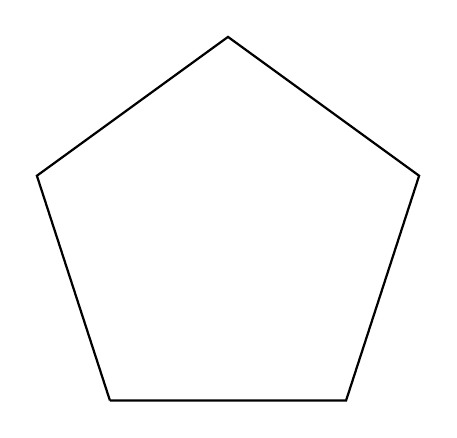
\begin{tikzpicture}[thick,scale=0.6]
    \draw (0,0) node{} -- (5,0) node{} -- ++(72:5) node{} -- ++(2*72:5) node{} -- ++(3*72:5) node{} -- (0,0);
  \end{tikzpicture}
\end{center}
\aln{
	y_1 + y_2 + y_3 + y_4 + y_5 - 5 &= 0\\
	y_1(y_1 - 1) &= 0\\
	y_2(y_2 - 1) &= 0\\
	y_3(y_3 - 1) &= 0\\
	y_4(y_4 - 1) &= 0\\
	y_5(y_5 - 1) &= 0\\
	(x_1 - 1)(x_1 - 2)(x_1 - 3)(x_1 - 4)(x_1 - 5) &= 0\\
	(x_2 - 1)(x_2 - 2)(x_2 - 3)(x_3 - 4)(x_2 - 5) &= 0\\
	(x_3 - 1)(x_3 - 2)(x_3 - 3)(x_3 - 4)(x_3 - 5) &= 0\\
	(x_4 - 1)(x_4 - 2)(x_4 - 3)(x_4 - 4)(x_4 - 5) &= 0\\
	(x_5 - 1)(x_5 - 2)(x_5 - 3)(x_5 - 4)(x_5 - 5) &= 0\\
	y_1 (x_1 - y_2 x_2 + y_2)(x_1 - y_2 x_2 - 4y_2)(x_1 - y_5 x_5 + y_5)(x_1 - y_5 x_5 - 4y_5) &= 0\\
	y_2 (x_2 - y_1 x_1 + y_1)(x_2 - y_1 x_1 - 4y_1)(x_2 - y_3 x_3 + y_3)(x_2 - y_3 x_3 - 4y_3) &= 0\\
	y_3 (x_3 - y_2 x_2 + y_2)(x_3 - y_2 x_2 - 4y_2)(x_3 - y_4 x_4 + y_4)(x_3 - y_4 x_4 - 4y_4) &= 0\\
	y_4 (x_4 - y_3 x_3 + y_3)(x_4 - y_3 x_3 - 4y_3)(x_4 - y_5 x_5 + y_5)(x_4 - y_5 x_5 - 4y_5) &= 0\\
	y_5 (x_5 - y_1 x_1 + y_1)(x_5 - y_1 x_1 - 4y_1)(x_5 - y_4 x_4 + y_4)(x_5 - y_4 x_4 - 4y_4) &= 0
}


\newpage

\section{Six Vertices with One Hamiltonian Cycle}
\begin{center}
  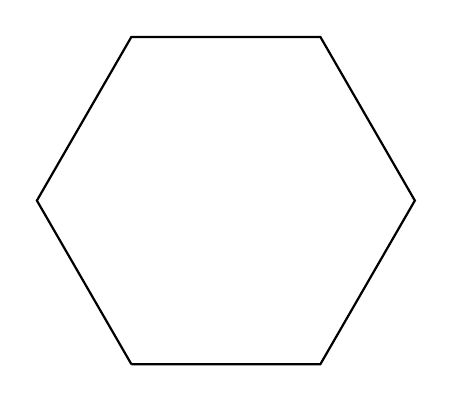
\begin{tikzpicture}[thick,scale=0.6]
    \draw (0,0) node{} -- (4,0) node{} -- ++(60:4) node{} -- ++(2*60:4) node{} -- ++(3*60:4) node{} -- ++(4*60:4) node{} -- (0,0);
  \end{tikzpicture}
\end{center}
\aln{
	y_1 + y_2 + y_3 + y_4 + y_5 + y_6 - 6 &= 0\\
	y_1(y_1 - 1) &= 0\\
	y_2(y_2 - 1) &= 0\\
	y_3(y_3 - 1) &= 0\\
	y_4(y_4 - 1) &= 0\\
	y_5(y_5 - 1) &= 0\\
	y_6(y_6 - 1) &= 0\\
	(x_1 - 1)(x_1 - 2)(x_1 - 3)(x_1 - 4)(x_1 - 5)(x_1 - 6) &= 0\\
	(x_2 - 1)(x_2 - 2)(x_2 - 3)(x_3 - 4)(x_2 - 5)(x_2 - 6) &= 0\\
	(x_3 - 1)(x_3 - 2)(x_3 - 3)(x_3 - 4)(x_3 - 5)(x_3 - 6) &= 0\\
	(x_4 - 1)(x_4 - 2)(x_4 - 3)(x_4 - 4)(x_4 - 5)(x_4 - 6) &= 0\\
	(x_5 - 1)(x_5 - 2)(x_5 - 3)(x_5 - 4)(x_5 - 5)(x_5 - 6) &= 0\\
	(x_6 - 1)(x_6 - 2)(x_6 - 3)(x_6 - 4)(x_6 - 5)(x_6 - 6) &= 0\\
	y_1 (x_1 - y_2 x_2 + y_2)(x_1 - y_2 x_2 - 5y_2)(x_1 - y_6 x_6 + y_6)(x_1 - y_6 x_6 - 5y_6) &= 0\\
	y_2 (x_2 - y_1 x_1 + y_1)(x_2 - y_1 x_1 - 5y_1)(x_2 - y_3 x_3 + y_3)(x_2 - y_3 x_3 - 5y_3) &= 0\\
	y_3 (x_3 - y_2 x_2 + y_2)(x_3 - y_2 x_2 - 5y_2)(x_3 - y_4 x_4 + y_4)(x_3 - y_4 x_4 - 5y_4) &= 0\\
	y_4 (x_4 - y_3 x_3 + y_3)(x_4 - y_3 x_3 - 5y_3)(x_4 - y_5 x_5 + y_5)(x_4 - y_5 x_5 - 5y_5) &= 0\\
	y_5 (x_5 - y_4 x_4 + y_4)(x_5 - y_4 x_4 - 5y_4)(x_5 - y_6 x_6 + y_6)(x_5 - y_6 x_6 - 5y_6) &= 0\\
	y_6 (x_6 - y_1 x_1 + y_1)(x_6 - y_1 x_1 - 5y_1)(x_6 - y_5 x_5 + y_5)(x_6 - y_5 x_5 - 5y_5) &= 0
}


\newpage

\section{Four Vertices with no Hamiltonian Cycles}
\begin{center}
  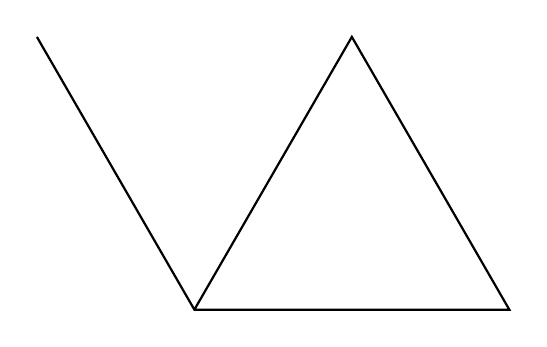
\begin{tikzpicture}[thick,scale=0.8]
    \draw (120:5) node{} -- (0,0) node{} -- (5,0) node{} -- (60:5) node{} -- (0,0);
  \end{tikzpicture}
\end{center}
\aln{
	y_1 + y_2 + y_3 + y_4 - 4 &= 0\\
	y_1(y_1 - 1) &= 0\\
	y_2(y_2 - 1) &= 0\\
	y_3(y_3 - 1) &= 0\\
	y_4(y_4 - 1) &= 0\\
	(x_1 - 1)(x_1 - 2)(x_1 - 3)(x_1 - 4) &= 0\\
	(x_2 - 1)(x_2 - 2)(x_2 - 3)(x_3 - 4) &= 0\\
	(x_3 - 1)(x_3 - 2)(x_3 - 3)(x_3 - 4) &= 0\\
	(x_4 - 1)(x_4 - 2)(x_4 - 3)(x_4 - 4) &= 0\\
	y_1 (x_1 - y_2 x_2 + y_2)(x_1 - y_2 x_2 - 3y_2) &= 0\\
	y_2 (x_2 - y_1 x_1 + y_1)(x_2 - y_1 x_1 - 3y_1)(x_2 - y_3 x_3 + y_3)(x_2 - y_3 x_3 - 3y_3) &= 0\\
	y_3 (x_3 - y_2 x_2 + y_2)(x_3 - y_2 x_2 - 3y_2)(x_3 - y_4 x_4 + y_4)(x_3 - y_4 x_4 - 3y_4) &= 0\\
	y_4 (x_4 - y_2 x_2 + y_1)(x_4 - y_2 x_2 - 3y_2)(x_4 - y_3 x_3 + y_3)(x_4 - y_3 x_3 - 3y_3) &= 0
}
\aln{
	\{1\}
}


\newpage

\section{Complete Graph with Four Vertices}
\begin{center}
  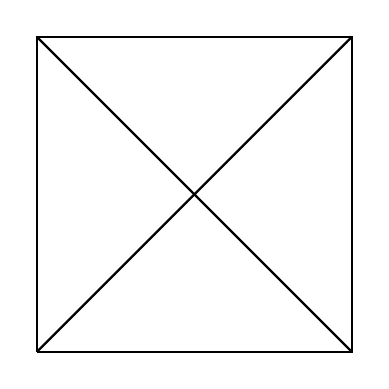
\begin{tikzpicture}[thick,scale=0.8]
    \draw (0,0) -- (5,5);
    \draw (5,0) -- (0,5);
    \draw (0,0) node {} -- (5,0) node {} -- (5,5) node {} -- (0,5) node {} -- (0,0);
  \end{tikzpicture}
\end{center}
\aln{
	y_1 + y_2 + y_3 + y_4 - 4 &= 0\\
	y_1(y_1 - 1) &= 0\\
	y_2(y_2 - 1) &= 0\\
	y_3(y_3 - 1) &= 0\\
	y_4(y_4 - 1) &= 0\\
	(x_1 - 1)(x_1 - 2)(x_1 - 3)(x_1 - 4) &= 0\\
	(x_2 - 1)(x_2 - 2)(x_2 - 3)(x_3 - 4) &= 0\\
	(x_3 - 1)(x_3 - 2)(x_3 - 3)(x_3 - 4) &= 0\\
	(x_4 - 1)(x_4 - 2)(x_4 - 3)(x_4 - 4) &= 0\\
	y_1 (x_1 - y_2 x_2 + y_2)(x_1 - y_2 x_2 - 3y_2)&\\(x_1 - y_3 x_3 + y_3)(x_1 - y_3 x_3 - 3y_3)(x_1 - y_4 x_4 + y_4)(x_1 - y_4 x_4 - 3y_4) &= 0\\
	y_2 (x_2 - y_1 x_1 + y_1)(x_2 - y_1 x_1 - 3y_1)&\\(x_2 - y_3 x_3 + y_3)(x_2 - y_3 x_3 - 3y_3)(x_2 - y_4 x_4 + y_4)(x_2 - y_4 x_4 - 3y_4) &= 0\\
	y_3 (x_3 - y_1 x_1 + y_1)(x_3 - y_1 x_1 - 3y_1)&\\(x_3 - y_2 x_2 + y_2)(x_3 - y_2 x_2 - 3y_2)(x_3 - y_4 x_4 + y_4)(x_3 - y_4 x_4 - 3y_4) &= 0\\
	y_4 (x_4 - y_1 x_1 + y_1)(x_4 - y_1 x_1 - 3y_1)&\\(x_4 - y_2 x_2 + y_2)(x_4 - y_2 x_2 - 3y_2)(x_4 - y_3 x_3 + y_3)(x_4 - y_3 x_3 - 3y_3) &= 0
}
\aln{
	\{&x_4^4-10x_4^3+35x_4^2-50x_4+24, x_3^3+x_3^2x_4-10x_3^2+x_3x_4^2-10x_3x_4+35x_3+x_4^3-10x_4^2+35x_4-50,\\& x_2^2+x_2x_3+x_2x_4-10x_2+x_3^2+x_3x_4-10x_3+x_4^2-10x_4+35, x_1+x_2+x_3+x_4-10,\\& y_4-1, y_3-1, y_2-1, y_1-1\}
}

\newpage

\section{Five Vertices with One Hamiltonian Cycle and Additional Edges}
\begin{center}
  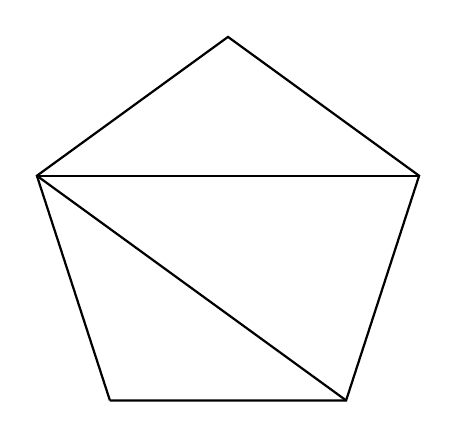
\begin{tikzpicture}[thick,scale=0.6]
    \draw (108:5) -- (5,0);
    \draw (5,0) ++(72:5) -- (108:5);
    \draw (0,0) node{} -- (5,0) node{} -- ++(72:5) node{} -- ++(2*72:5) node{} -- ++(3*72:5) node{} -- (0,0);
  \end{tikzpicture}
\end{center}
\aln{
	y_1 + y_2 + y_3 + y_4 + y_5 - 5 &= 0\\
	y_1(y_1 - 1) &= 0\\
	y_2(y_2 - 1) &= 0\\
	y_3(y_3 - 1) &= 0\\
	y_4(y_4 - 1) &= 0\\
	y_5(y_5 - 1) &= 0\\
	(x_1 - 1)(x_1 - 2)(x_1 - 3)(x_1 - 4)(x_1 - 5) &= 0\\
	(x_2 - 1)(x_2 - 2)(x_2 - 3)(x_3 - 4)(x_2 - 5) &= 0\\
	(x_3 - 1)(x_3 - 2)(x_3 - 3)(x_3 - 4)(x_3 - 5) &= 0\\
	(x_4 - 1)(x_4 - 2)(x_4 - 3)(x_4 - 4)(x_4 - 5) &= 0\\
	(x_5 - 1)(x_5 - 2)(x_5 - 3)(x_5 - 4)(x_5 - 5) &= 0\\
	y_1 (x_1 - y_2 x_2 + y_2)(x_1 - y_2 x_2 - 4y_2)(x_1 - y_5 x_5 + y_5)(x_1 - y_5 x_5 - 4y_5) &= 0\\
	y_2 (x_2 - y_1 x_1 + y_1)(x_2 - y_1 x_1 - 4y_1)(x_2 - y_3 x_3 + y_3)(x_2 - y_3 x_3 - 4y_3)(x_2 - y_5 x_5 + y_5)(x_2 - y_5 x_5 - 4y_5) &= 0\\
	y_3 (x_3 - y_2 x_2 + y_2)(x_3 - y_2 x_2 - 4y_2)(x_3 - y_4 x_4 + y_4)(x_3 - y_4 x_4 - 4y_4)(x_3 - y_5 x_5 + y_5)(x_3 - y_5 x_5 - 4y_5) &= 0\\
	y_4 (x_4 - y_3 x_3 + y_3)(x_4 - y_3 x_3 - 4y_3)(x_4 - y_5 x_5 + y_5)(x_4 - y_5 x_5 - 4y_5) &= 0\\
	y_5 (x_5 - y_1 x_1 + y_1)(x_5 - y_1 x_1 - 4y_1)(x_5 - y_2 x_2 + y_2)(x_5 - y_2 x_2 - 4y_2)(x_5 - y_3 x_3 + y_3)(x_5 - y_3 x_3 - 4y_3)(x_5 - y_4 x_4 + y_4)(x_5 - y_4 x_4 - 4y_4) &= 0
}


\newpage

\section{Five Vertices with Multiple Hamiltionian Cycles}
\begin{center}
  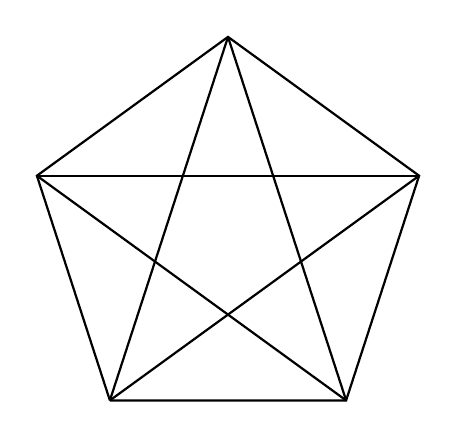
\begin{tikzpicture}[thick,scale=0.6]
    \draw (5,0)++(72:5) -- (0,0);
    \draw (5,0)++(72:5)++(2*72:5) -- (0,0);
    \draw (5,0)++(72:5)++(2*72:5) -- (5,0);
    \draw (108:5) -- (5,0);
    \draw (5,0) ++(72:5) -- (108:5);
    \draw (0,0) node{} -- (5,0) node{} -- ++(72:5) node{} -- ++(2*72:5) node{} -- ++(3*72:5) node{} -- (0,0);
  \end{tikzpicture}
\end{center}
\aln{
	y_1 + y_2 + y_3 + y_4 + y_5 - 5 &= 0\\
	y_1(y_1 - 1) &= 0\\
	y_2(y_2 - 1) &= 0\\
	y_3(y_3 - 1) &= 0\\
	y_4(y_4 - 1) &= 0\\
	y_5(y_5 - 1) &= 0\\
	(x_1 - 1)(x_1 - 2)(x_1 - 3)(x_1 - 4)(x_1 - 5) &= 0\\
	(x_2 - 1)(x_2 - 2)(x_2 - 3)(x_3 - 4)(x_2 - 5) &= 0\\
	(x_3 - 1)(x_3 - 2)(x_3 - 3)(x_3 - 4)(x_3 - 5) &= 0\\
	(x_4 - 1)(x_4 - 2)(x_4 - 3)(x_4 - 4)(x_4 - 5) &= 0\\
	(x_5 - 1)(x_5 - 2)(x_5 - 3)(x_5 - 4)(x_5 - 5) &= 0\\
	y_1 (x_1 - y_2 x_2 + y_2)(x_1 - y_2 x_2 - 4y_2)(x_1 - y_3 x_3 + y_3)(x_1 - y_3 x_3 - 4y_3)(x_1 - y_4 x_4 + y_4)(x_1 - y_4 x_4 - 4y_4)(x_1 - y_5 x_5 + y_5)(x_1 - y_5 x_5 - 4y_5) &= 0\\
	y_2 (x_2 - y_1 x_1 + y_1)(x_2 - y_1 x_1 - 4y_1)(x_2 - y_3 x_3 + y_3)(x_2 - y_3 x_3 - 4y_3)(x_2 - y_4 x_4 + y_4)(x_2 - y_4 x_4 - 4y_4)(x_2 - y_5 x_5 + y_5)(x_2 - y_5 x_5 - 4y_5) &= 0\\
	y_3 (x_3 - y_1 x_1 + y_1)(x_3 - y_1 x_1 - 4y_1)(x_3 - y_2 x_2 + y_2)(x_3 - y_2 x_2 - 4y_2)(x_3 - y_4 x_4 + y_4)(x_3 - y_4 x_4 - 4y_4)(x_3 - y_5 x_5 + y_5)(x_3 - y_5 x_5 - 4y_5) &= 0\\
	y_4 (x_4 - y_1 x_1 + y_1)(x_4 - y_1 x_1 - 4y_1)(x_4 - y_2 x_2 + y_2)(x_4 - y_2 x_2 - 4y_2)(x_4 - y_3 x_3 + y_3)(x_4 - y_3 x_3 - 4y_3)(x_4 - y_5 x_5 + y_5)(x_4 - y_5 x_5 - 4y_5) &= 0\\
	y_5 (x_5 - y_1 x_1 + y_1)(x_5 - y_1 x_1 - 4y_1)(x_5 - y_2 x_2 + y_2)(x_5 - y_2 x_2 - 4y_2)(x_5 - y_3 x_3 + y_3)(x_5 - y_3 x_3 - 4y_3)(x_5 - y_4 x_4 + y_4)(x_5 - y_4 x_4 - 4y_4) &= 0
}


\newpage

\section{Six Vertices with Multiple Hamiltonian Cycles (4-Regular)}
\begin{center}
  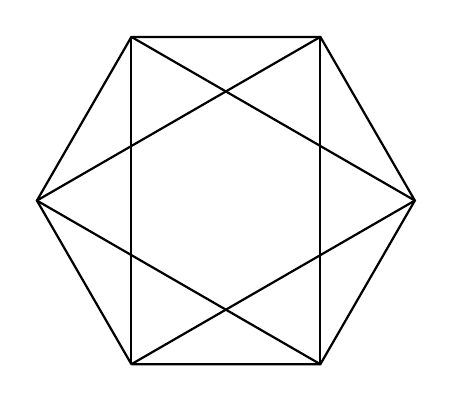
\begin{tikzpicture}[thick,scale=0.6]
    \draw (4,0)++(60:4) -- (0,0);
    \draw (4,0)++(60:4)++(2*60:4)++(3*60:4) -- (0,0);
    \path (4,0)++(60:4)++(2*60:4)++(3*60:4) coordinate(farpoint);
    \draw (4,0)++(60:4) -- (farpoint);
    \draw (4,0)++(60:4)++(2*60:4) -- (4,0);
    \draw (4,0)++(60:4)++(2*60:4) -- (120:4);
    \draw (120:4) -- (4,0);
    \draw (0,0) node{} -- (4,0) node{} -- ++(60:4) node{} -- ++(2*60:4) node{} -- ++(3*60:4) node{} -- ++(4*60:4) node{} -- (0,0);
  \end{tikzpicture}
\end{center}
\aln{
	y_1 + y_2 + y_3 + y_4 + y_5 + y_6 - 6 &= 0\\
	y_1(y_1 - 1) &= 0\\
	y_2(y_2 - 1) &= 0\\
	y_3(y_3 - 1) &= 0\\
	y_4(y_4 - 1) &= 0\\
	y_5(y_5 - 1) &= 0\\
	y_6(y_6 - 1) &= 0\\
	(x_1 - 1)(x_1 - 2)(x_1 - 3)(x_1 - 4)(x_1 - 5)(x_1 - 6) &= 0\\
	(x_2 - 1)(x_2 - 2)(x_2 - 3)(x_3 - 4)(x_2 - 5)(x_2 - 6) &= 0\\
	(x_3 - 1)(x_3 - 2)(x_3 - 3)(x_3 - 4)(x_3 - 5)(x_3 - 6) &= 0\\
	(x_4 - 1)(x_4 - 2)(x_4 - 3)(x_4 - 4)(x_4 - 5)(x_4 - 6) &= 0\\
	(x_5 - 1)(x_5 - 2)(x_5 - 3)(x_5 - 4)(x_5 - 5)(x_5 - 6) &= 0\\
	(x_6 - 1)(x_6 - 2)(x_6 - 3)(x_6 - 4)(x_6 - 5)(x_6 - 6) &= 0\\
	y_1 (x_1 - y_2 x_2 + y_2)(x_1 - y_2 x_2 - 5y_2)(x_1 - y_3 x_3 + y_3)(x_1 - y_3 x_3 - 5y_3)(x_1 - y_5 x_5 + y_5)(x_1 - y_5 x_5 - 5y_5)(x_1 - y_6 x_6 + y_6)(x_1 - y_6 x_6 - 5y_6) &= 0\\
	y_2 (x_2 - y_1 x_1 + y_1)(x_2 - y_1 x_1 - 5y_1)(x_2 - y_3 x_3 + y_3)(x_2 - y_3 x_3 - 5y_3)(x_2 - y_4 x_4 + y_4)(x_2 - y_4 x_4 - 5y_4)(x_2 - y_6 x_6 + y_6)(x_2 - y_6 x_6 - 5y_6) &= 0\\
	y_3 (x_3 - y_1 x_1 + y_1)(x_3 - y_1 x_1 - 5y_1)(x_3 - y_2 x_2 + y_2)(x_3 - y_2 x_2 - 5y_2)(x_3 - y_4 x_4 + y_4)(x_3 - y_4 x_4 - 5y_4)(x_3 - y_5 x_5 + y_5)(x_3 - y_5 x_5 - 5y_5) &= 0\\
	y_4 (x_4 - y_2 x_2 + y_2)(x_4 - y_2 x_2 - 5y_2)(x_4 - y_3 x_3 + y_3)(x_4 - y_3 x_3 - 5y_3)(x_4 - y_5 x_5 + y_5)(x_4 - y_5 x_5 - 5y_5)(x_4 - y_6 x_6 + y_6)(x_4 - y_6 x_6 - 5y_6) &= 0\\
	y_5 (x_5 - y_1 x_1 + y_1)(x_5 - y_1 x_1 - 5y_1)(x_5 - y_3 x_3 + y_3)(x_5 - y_3 x_3 - 5y_3)(x_5 - y_4 x_4 + y_4)(x_5 - y_4 x_4 - 5y_4)(x_5 - y_6 x_6 + y_6)(x_5 - y_6 x_6 - 5y_6) &= 0\\
	y_6 (x_6 - y_1 x_1 + y_1)(x_6 - y_1 x_1 - 5y_1)(x_6 - y_2 x_2 + y_2)(x_6 - y_2 x_2 - 5y_2)(x_6 - y_4 x_4 + y_4)(x_6 - y_4 x_4 - 5y_4)(x_6 - y_5 x_5 + y_5)(x_6 - y_5 x_5 - 5y_5) &= 0
}


\newpage

\section{Six Vertices with Multiple Hamiltonian Cycles (5-Regular)}
\begin{center}
  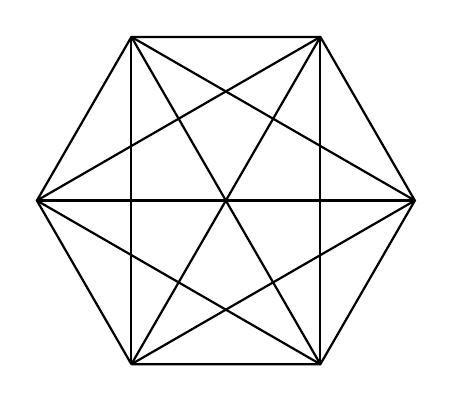
\begin{tikzpicture}[thick,scale=0.6]
    \draw (4,0)++(60:4) -- (0,0);
    \draw (4,0)++(60:4)++(2*60:4)++(3*60:4) -- (0,0);
    \path (4,0)++(60:4)++(2*60:4)++(3*60:4) coordinate(farpoint);
    \draw (4,0)++(60:4) -- (farpoint);
    \draw (4,0)++(60:4)++(2*60:4) -- (4,0);
    \draw (4,0)++(60:4)++(2*60:4) -- (120:4);
    \draw (120:4) -- (4,0);
    \draw (4,0)++(60:4)++(2*60:4) -- (0,0);
    \draw (4,0)++(60:4) -- (120:4);
    \draw (4,0)++(60:4)++(2*60:4)++(3*60:4) -- (4,0);
    \draw (0,0) node{} -- (4,0) node{} -- ++(60:4) node{} -- ++(2*60:4) node{} -- ++(3*60:4) node{} -- ++(4*60:4) node{} -- (0,0);
  \end{tikzpicture}
\end{center}
\aln{
	y_1 + y_2 + y_3 + y_4 + y_5 + y_6 - 6 &= 0\\
	y_1(y_1 - 1) &= 0\\
	y_2(y_2 - 1) &= 0\\
	y_3(y_3 - 1) &= 0\\
	y_4(y_4 - 1) &= 0\\
	y_5(y_5 - 1) &= 0\\
	y_6(y_6 - 1) &= 0\\
	(x_1 - 1)(x_1 - 2)(x_1 - 3)(x_1 - 4)(x_1 - 5)(x_1 - 6) &= 0\\
	(x_2 - 1)(x_2 - 2)(x_2 - 3)(x_3 - 4)(x_2 - 5)(x_2 - 6) &= 0\\
	(x_3 - 1)(x_3 - 2)(x_3 - 3)(x_3 - 4)(x_3 - 5)(x_3 - 6) &= 0\\
	(x_4 - 1)(x_4 - 2)(x_4 - 3)(x_4 - 4)(x_4 - 5)(x_4 - 6) &= 0\\
	(x_5 - 1)(x_5 - 2)(x_5 - 3)(x_5 - 4)(x_5 - 5)(x_5 - 6) &= 0\\
	(x_6 - 1)(x_6 - 2)(x_6 - 3)(x_6 - 4)(x_6 - 5)(x_6 - 6) &= 0\\
	y_1 (x_1 - y_2 x_2 + y_2)(x_1 - y_2 x_2 - 5y_2)(x_1 - y_3 x_3 + y_3)(x_1 - y_3 x_3 - 5y_3)(x_1 - y_4 x_4 + y_4)(x_1 - y_4 x_4 - 5y_4)(x_1 - y_5 x_5 + y_5)(x_1 - y_5 x_5 - 5y_5)(x_1 - y_6 x_6 + y_6)(x_1 - y_6 x_6 - 5y_6) &= 0\\
	y_2 (x_2 - y_1 x_1 + y_1)(x_2 - y_1 x_1 - 5y_1)(x_2 - y_3 x_3 + y_3)(x_2 - y_3 x_3 - 5y_3)(x_2 - y_4 x_4 + y_4)(x_2 - y_4 x_4 - 5y_4)(x_2 - y_5 x_5 + y_5)(x_2 - y_5 x_5 - 5y_5)(x_2 - y_6 x_6 + y_6)(x_2 - y_6 x_6 - 5y_6) &= 0\\
	y_3 (x_3 - y_1 x_1 + y_1)(x_3 - y_1 x_1 - 5y_1)(x_3 - y_2 x_2 + y_2)(x_3 - y_2 x_2 - 5y_2)(x_3 - y_4 x_4 + y_4)(x_3 - y_4 x_4 - 5y_4)(x_3 - y_5 x_5 + y_5)(x_3 - y_5 x_5 - 5y_5)(x_3 - y_6 x_6 + y_6)(x_3 - y_6 x_6 - 5y_6) &= 0\\
	y_4 (x_4 - y_1 x_1 + y_1)(x_4 - y_1 x_1 - 5y_1)(x_4 - y_2 x_2 + y_2)(x_4 - y_2 x_2 - 5y_2)(x_4 - y_3 x_3 + y_3)(x_4 - y_3 x_3 - 5y_3)(x_4 - y_5 x_5 + y_5)(x_4 - y_5 x_5 - 5y_5)(x_4 - y_6 x_6 + y_6)(x_4 - y_6 x_6 - 5y_6) &= 0\\
	y_5 (x_5 - y_1 x_1 + y_1)(x_5 - y_1 x_1 - 5y_1)(x_5 - y_2 x_2 + y_2)(x_5 - y_2 x_2 - 5y_2)(x_5 - y_3 x_3 + y_3)(x_5 - y_3 x_3 - 5y_3)(x_5 - y_4 x_4 + y_4)(x_5 - y_4 x_4 - 5y_4)(x_5 - y_6 x_6 + y_6)(x_5 - y_6 x_6 - 5y_6) &= 0\\
	y_6 (x_6 - y_1 x_1 + y_1)(x_6 - y_1 x_1 - 5y_1)(x_6 - y_2 x_2 + y_2)(x_6 - y_2 x_2 - 5y_2)(x_6 - y_3 x_3 + y_3)(x_6 - y_3 x_3 - 5y_3)(x_6 - y_4 x_4 + y_4)(x_6 - y_4 x_4 - 5y_4)(x_6 - y_5 x_5 + y_5)(x_6 - y_5 x_5 - 5y_5) &= 0
}



\end{document}
